\section{Timeline for project}
This semester project can be split into 6 parts, as seen on \autoref{fig:timeline-for-project}
There are 4 sprints for developing the application. 
As PO or scrum group there are a lot of work preparing for the first sprint.
This is what we consider "Pre sprint 1" and after that there are 4 sprints for developing the weekplanner.
The process group planned so that the last sprint will end 2 weeks before the deadline of handing in the project.
These last two weeks are spend on usability test with the customers and finishing the report.
What is common for every sprint is that they follow the scrum of scrum guidelines previous described ín \autoref{scrum-of-scrums}.

\begin{figure}[H]
    \center{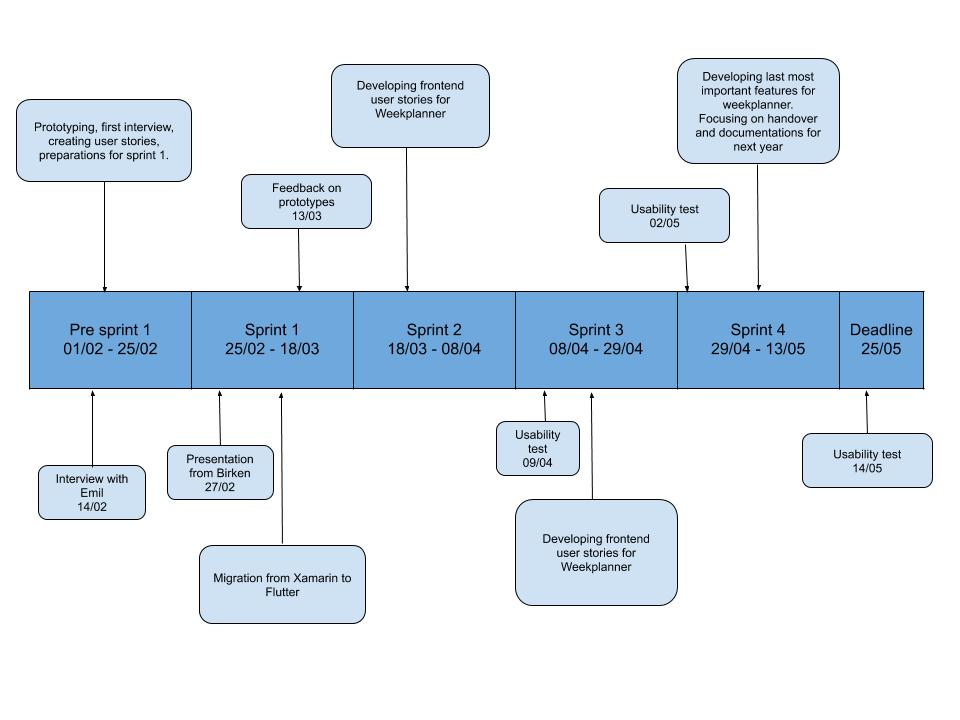
\includegraphics[width=\textwidth]
    {figures/timeline-for-entire-project.JPG}}
    \caption{\label{fig:timeline-for-project} Timeline for the project.}
\end{figure}

\todo{Figure is updated continously}

\subsubsection{Pre sprint 1}
There was pre sprint 1, where the preparation for sprint 1 happend.
During this time the POs contact and interview customers to gain insight on what is wanted by the customers.
With these interviews user stories and prototypes are created so that they are ready for sprint 1.
In pre sprint 1 an interview with Emil from Egebakken was conducted. 
This interview is described in \autoref{interview-with-emil}.

\subsubsection{Sprint 1}
February the 27th there were a presentation from the kintergarden Birken.
This presentation is described in \autoref{presentation-from-birken}.
The focus of this sprint started out being towards fixing bugs and stabilizing the application.
It turned out that there were a lot of problems with the frontend with Xamarin and was decided to migrate the frontend to Flutter.
This pros and cons for the decision is described in \autoref{change-of-framework}.
This also resulted in the PO needing to look into the user stories, as new user stories for previously implemented features needed to be implemented again and many of the old user stories had to gain a lower priority.
A meeting was planned with the customers March 13th to get feedback on the prototypes. 
This interview resulted in some of the prototypes getting reworked to better fit with the customers needs.


\subsubsection{Sprint 2}
As there were no release at the end of sprint 1 because of the desicion to migrate to flutter, there were not conducted a usability test.
Instead this sprint were used on developing user stories planned in sprint 1.


\todo{To be continued...}

\subsubsection{Sprint 3}
\todo{Write in sprint 3}

\subsubsection{Sprint 4}
\todo{Write in sprint 4}
\subsubsection{Deadline}
\todo{Write after usability test after sprint 4.}
